\documentclass[a4paper]{article}
\usepackage[utf8]{inputenc}
\usepackage[T1]{fontenc}
\usepackage{graphicx}
\usepackage{hyperref}
\usepackage[english]{babel}
\usepackage[super]{nth}
\usepackage{fancyhdr}
\usepackage{tabu}
\usepackage{multirow}
\usepackage{cite}
\usepackage{amsmath}


\DeclareGraphicsExtensions{.pdf,.png,.jpg,.eps}

\newcommand{\mytitle}{Zombie Apocalypse Report}
\newcommand*\mean[1]{\overline{#1}}

\pagestyle{fancy}
\fancyhf{}
\fancyhead[L]{Juraszek, Shiong, Signorini, Yang}
\fancyhead[R]{\mytitle}

\fancyfoot[C]{\thepage}

\title{\mytitle}
\author{Adam Juraszek \and Ryan Leong Wei Shiong \and Matthew Signorini \and Ziying Yang}

\begin{document}
\maketitle

\section{Introduction} % Ryan

Infectious diseases have been prevalent since the start of time.
Modelling the spread of these diseases can serve to find possible ways to stop or limit the spreading.
With the advancement of technology, computing power has increased tremendously, allowing these simulation models to be done on a greater scale.
In this project, we are to implement a Zombie Infection simulation, modeling the spread of the infection on a human population.
The entities in the simulation are split into three main categories, Humans, Infected and Zombies.
Infected are humans which will eventually turn into Zombies.

\subsection{Zombie description}

Since this is a, currently, fictional situation, the various different literatures provide different zombie characteristics.
For an instance, an article on the zombies of ``World War Z'', the zombies in the lore are slow moving until they sense humans around.
They will then move as fast, if not, faster than human running speed. \cite{guidetozombies}

In our model, the zombies are reanimated dead human bodies controlled by a viral infection, which is one of known types of zombies. \cite{survivingthedead}
A human becomes infected when it is bitten by a zombie.
The infection doesn't have any symptoms except for bite marks and short term memory loss.
The infection is latent and secretly spreads inside the body until it dominates.
The incubation period is 14 days on average, which is significantly longer than we are accustomed, however it has a medical support. \cite{mogk2011everything}
Later, during a weak moment (usually while sleeping) it causes death of the person and starts act on its own.

The zombies are naturally strongly atracted to humans to infect them and humans run away from zombies when they spot them.
The control of the body is poor and therefore the movement and motorics is slower and inaccurate.
The durability period of a reanimated dead body is shortend to about 3 years on average. \cite{zombiepedia}
Eventually a zombie falls and decomposes.

\subsection{Requirements}

\begin{enumerate}
\item In the first part of this project, the task was to simulate the human and zombie population on a 500 by 500 grid.
\item We had to take into account the birth and death rate of humans, keeping them close to the current demographics of the Northern Territory in Australia.
    This hold except for the population size which is reduced to one half. \cite{project}
\item We had to model zombies which are eager to chase and infect humans.
    We had to model zombie processes starting with infection and ending with decomposition.
\item With this model, we aim to find parameters which support coexisting of both populations of humans and zombies, and also don't contradict reality.
\end{enumerate}

\subsubsection{Stability requirement}

The last requirment makes the model hard as we cannot allow either population to drop too low and, as a consequence, to rise too high either.
If there were too little humans, the zombies couldn't infect anybody often enough to compensate their shorter lifespan.
On the other hand, if there are too many humans, the infection can spread very quickly and the zombies outnumber humans.
This is followed by steep decrease of both populations and finally becomes the former case with possibility of humans extinction.

\section{Model} % Adam

\subsection{Infection model}

\begin{figure*}[ht]
        \centering
        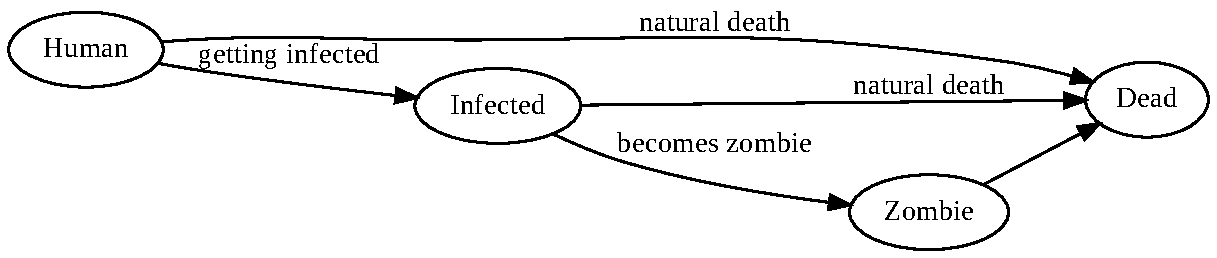
\includegraphics[width=\textwidth]{model}
        \caption{Infection model}
\end{figure*}

Since we don't suppose that there has not been found cure for infected (nor zombies) to become humans again, our model presumes only four possible stages and strictly one-way transitions.
This and non-existence of immunity is the main difference between our model and clasic SIR model and its variations.

An entity begins in state Human which represents a normal human being which was born, has a gender (is either male or female), and eventually dies.
If a human gets in contact with a zombie, it may become infected.
The probability of infection is unknown but for the purpose of our model it was set to $0.75\%$ for a human within 1 kilometer proximity to a zombie.
However small the probablility seems to be, it is quite acceptable concerning the smallest time and space units being 1 day and 1 kilometer.

Infected entity is basically a human which eventually becomes a zombie that means it can reproduce and die of natural death.
Infected entity is not a danger to the surrounding humans until it becomes a zombie.
Zombie is concidered death -- it is just a virus-driven moving body; therefore we say that a zombie eventually decomposes insead of it dies.
In our model, zombie doesn't have gender as it cannot reproduce nor its properties depend on gender of the human which it used to be.

When a human becomes infected, the length of the infection depends on the strength of the body fighting the zombie virus.
The transition happens with a certain probability that makes the average length of infection 14 days.

\subsubsection{Reproduction}

If two fertile living entities (no matter if humans infected) of different genders meet, they can make love and conceive a baby.
It takes approximately 9 months for a child to develop inside mother's womb before it is born. \cite{pregnancy}
As the zombies are of viral nature, we presume that the virus in infected mother's body is passed to unborn children.
The virus is not transmitted when an infected has an intercourse with a healthy human.

A female can become pregnant if she is not already pregnant, and she is in a fertile age (roughtly between 15 and 45 years) and her partner is a male in a fertile age (roughtly between 15 and 80).
More than one baby can be conceived during one intercourse -- our model supports that a female can expect up to three babies at once.
The probabilities of multiple births are in accordance with Hellin's law. \cite{hellinslaw}

\subsubsection{Age}

The model follows the Australian age distribution for both males and females.
When the simulation starts, the humans are divided into age classes based on their actual age.
Within an age class, the people are distributed uniformly.

Humans and infected are sorted into four age classes:
\begin{enumerate}
\item a child (0--15 years),
\item young (15--37.5 years),
\item middle aged (37.5--65 years),
\item elderly (65+).
\end{enumerate}

According to the latest scientific research, zombies live 3 to 5 years. \cite{zombiepedia}
Zombies are divided into two age classes:
\begin{enumerate}
\item young (0--1.5 years),
\item old (1.5+).
\end{enumerate}

Most of the properties of the entities are dependent on their gender and on age class rather than on their actual age.
The properties are:
\begin{itemize}
\item daily death rate -- the probability of a natural death per each day,
\item speed -- the probability of the entity to leave its current cell if it was its original intension.
\end{itemize}

Since the moving speed is a probability and the cell size is enormous, it only makes sense to compare the probabilities.
Females are slightly slower but still faster than zombies.
Speed of a young zombie equals to speed of an elderly human male.

Details about death probabilities are discusses later in the report.

\subsection{World representation}

The final simulated world will be a mesh of size $1000 \times 1500$ which correspond with size of Northern Territory. \cite{northernterritory}
Parts of the mesh are called cells.
On each cell, there may be at most one entity of any type; otherwise the cell is considered empty.
Adjacency of two entities means that the two entities are touching each other, sharing one side of their cells.
The simulated world has fixed boundaries, no entity can pass through them; this is often refered as to no-flux boundary condition.

For the purpose of this report, only part of the world is simulated.
The actual size of the mesh is $500 \times 500$ cells.

\subsubsection{Movement}

\begin{figure*}[ht]
    \centering
    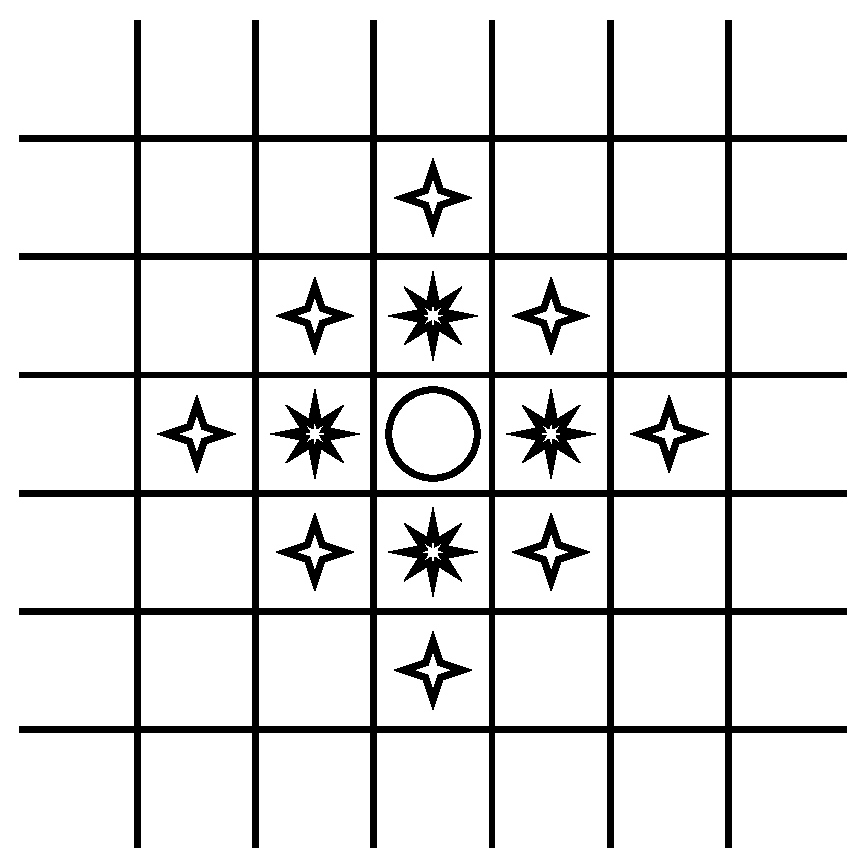
\includegraphics[width=0.3\textwidth]{movement}
    \caption{Considered cells when planning movement}
\end{figure*}

\begin{figure*}[ht]
    \centering
    \begin{tabu} {| X[1.8,c,p] || X[1,c,p] | X[1,c,p] | X[1,c,p] | X[1,c,p] | X[1.2,c,p] |}
        \rowfont{\bfseries}
        \hline
        sees &
        Wall &
        Empty tile&
        Zombie &
        Same gender &
        Opposite gender \\
        \hline
        \hline
        \textbf{Living entity} & -- & + & -- & + & ++ \\
        \hline
        \textbf{Zombie} & -- & + & + & \multicolumn{2}{c|}{ ++ } \\
        \hline
    \end{tabu}
    \caption{Affinity to directed situations for each type}
\end{figure*}

All entities, including zombies, share the same movement planning model.
They differ mainly in preference where to go.

Each entity determines its optimal direction based on surrounding 12 cells as shown on the diagram.
The cells to which it can get within one move are marked with a fancy star; cells accessible within two moves are marked with a simple star.
When considering directions, the adjacent cells always have higher priority.

Each entity rates each of these cells based on their content.
The preference for direction is then calculated as a weighted sum of complex numbers corresponding to particular directions.
The values of preference were chosen to mimic expected bahaviour.
Better results could be achieved by a more sophisticated (genetic) algorithm or by a more thorough analysis.
The current estimates can be seen in the table below.
To the current preffered direction the potential direction of the last move is added, that simulates inertia of movement and as a result it makes the movement targeted.

After the optimal weighted direction is calculated, it is translated to a particular direction, or stay instruction if the absolute value is not sufficient.
The direction may randomly change clock-wise or counter-clock-wise simulating evading obstacles, which are not modeled in the world.
Then the cell in the resulting direction is tested whether it is free; if it is not, the clock-wise or cunter-clock-wise one is chosen.
In the worst case, the entity stays at its current tile.
The entity moves only if its speed (expressed as probability) is sufficient.

\subsection{Initialisation of the population}

\subsubsection{Age structure and death rate}

\begin{figure*}[ht]
    \centering
    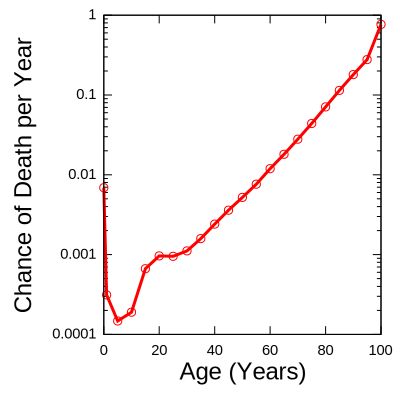
\includegraphics[width=0.6\textwidth]{USGompertzCurve}
    \caption{Mortality rates for US in 2003}
\end{figure*}

According to the Australian age structure\cite{agestructure} and median of age 37.3 years \cite{demographicsaustralia}, initialized humans are divided into four age clasess.
Based on Gompertz–Makeham law \cite{mortalitylaw} and mortality rates graph for US in 2003 (shown in the figure) the average probabilities of a human dying in these four age stages are approximately related as 
$$ \mean{P(\text{Elder Death})} = 10\: \mean{P(\text{Middle Age Death})} $$
$$ = 80\: \mean{P(\text{Young Death})} = 160\: \mean{P(\text{Child Death})} $$

As the Australian death rate \cite{absdeath} is
$$ \mean{P(\text{Australia Death})} = \frac{\text{people who died (in 2012)}}{\text{population size (in 2012)}} $$
$$ = \frac{147098}{23319400} = 0.63\%/\text{year} = 0.0017\%/\text{day} $$

The death rates for each age class can be calculated and expresses as shown in the table below.

\begin{figure*}[ht]
    \centering
    \begin{tabu} {| X[1.1,c,p] || X[0.7,c,p] | X[1.2,c,p] | X[1.1,c,p] | X[1,c,p] |}
        \rowfont{\bfseries}
        \hline
        Class Name &
        Age Range &
        Distribution &
        Average Death Rate (per day) &
        Death Rate (per day) \\
        \hline
        \hline
        \textbf{Child} & 0--15 & 18.2\% & \multirow{4}{*}{0.0017\%} & 0.00006\% \\
        \cline{1-3}\cline{5-5}
        \textbf{Young} & 15--37.5 & 31.8\% & & 0.00012\% \\
        \cline{1-3}\cline{5-5}
        \textbf{Middle Age} & 37.5--65 & 35.6\% & & 0.00096\% \\
        \cline{1-3}\cline{5-5}
        \textbf{Elderly} & 65+ & 14.4\% & & 0.0096\% \\
        \hline
    \end{tabu}
    \caption{Death rate of age classes}
\end{figure*}

\subsubsection{Birth rate}

There are two situations when the birth rate is used in a way.

First, when the simulation starts, some females should be pregnant.
The estimated probability of a female in fertility period being pregnant is:
$$ P(\text{Pregnant Female in Fertility Period}) $$
$$ = \frac{\text{average number of children per female life} \times \text{pregnancy duration}}{\text{average length of fertility period}} $$
$$ = \frac{1.77 \times 9 (\text{months})}{30 (\text{years})} = 4.36\% $$

Although we had access to birth rates, we didn't try to untilise them during the simulation because of the excessive difficulty of calculations.
Simple approach of counting probabilities of a male-female couples on a mesh do not work when the movement is targeted (as discussed earlier).
We also model fertilisation and pregnancy periods which naturally limit the baby procreation.

Our approach is to run the simulation of them model for several generations without presence of zombies, and by trials and errors find the right rate when the population size is stable or slightly increasing.
That way we got a probability of child being conceived each time a couple makes love equal to 0.00073, which is a number that doesn't make sense without context of the implemented model.
This is just a small price for much more realistic model of child birth.

\subsubsection{Sex ratio}

The birth ratio between males and females is 1.06. \cite{cia}
Thus the ratio of a child being a male of female is initialized as
$$ \text{Male Child} : \text{Female Child} = 0.5146 : 0.4854 $$

However, the ratio is different when the simulation starts.
The ratio in Australia is currently 1.01 and can be expressed as \cite{cia}
$$ \text{Male} : \text{Female} = 0.5025 : 0.4975 $$

\subsubsection{Population Density}

The population density in the Northern Territory prior to the zombie apocalypse is $0.17/\text{km}^2$. \cite{northernterritory}
When the viral infection starts, the authorities estimate that approximately half of the population will move from Australia to Sweden. \cite{project}
As the simulated mesh is $500 \times 500$, the initial number of simulated humans is
$$ 500 \cdot 500 \cdot \frac{0.17}{2} = 21250 $$

\section{Results}

Before presenting the actual results, we would like to describe an intermediate model which contained a flaw which made it stable.

\subsection{A flaw and its consequences}

When implementing the simulation of entities movement on a 2D mesh, we chose to use two nested for loops (the outer went through columns, the inner through rows) copying entities from the input mesh to the outer one.
For each entity the optimal decision where to move was calculated (as discussed earlier) and then tested whether the destination cell is free.
Unfortunatelly the chosen directino of processing causes that the cells to the left and to the up are already processed and there exists a chance that those cells will contain an entity.
On the other hand, the cells to the right and to the down are unprocessed and therefore the conflict is less likely.
This slight inequality causes that the overall movement is targeted to right and down and clusters of entities appear the the world border.

These clusters proved to be important for zombies.
It is an ideal place where they can feastand keep their number high untill the rest of the world regenerate.
They are also often places where the infection starts and spreads very quickly with creating a lot of zombies.

When the flaw was repaired (by randomizing the processing directions), the zombies could not survive under the previously stable conditions.
No matter what changes we did to the model, the infection probability had to be lowered from original value 0.01 to 0.0075.
The new probability keeps the zombie population size of at least 100 individuals at all time.

\subsection{Population size}

Making the model stable without zombies was easy.
In order to add zombies we had to change the model a bit to deal with zombies and their dynamic population size.

\begin{figure*}[pht]
    \centering
    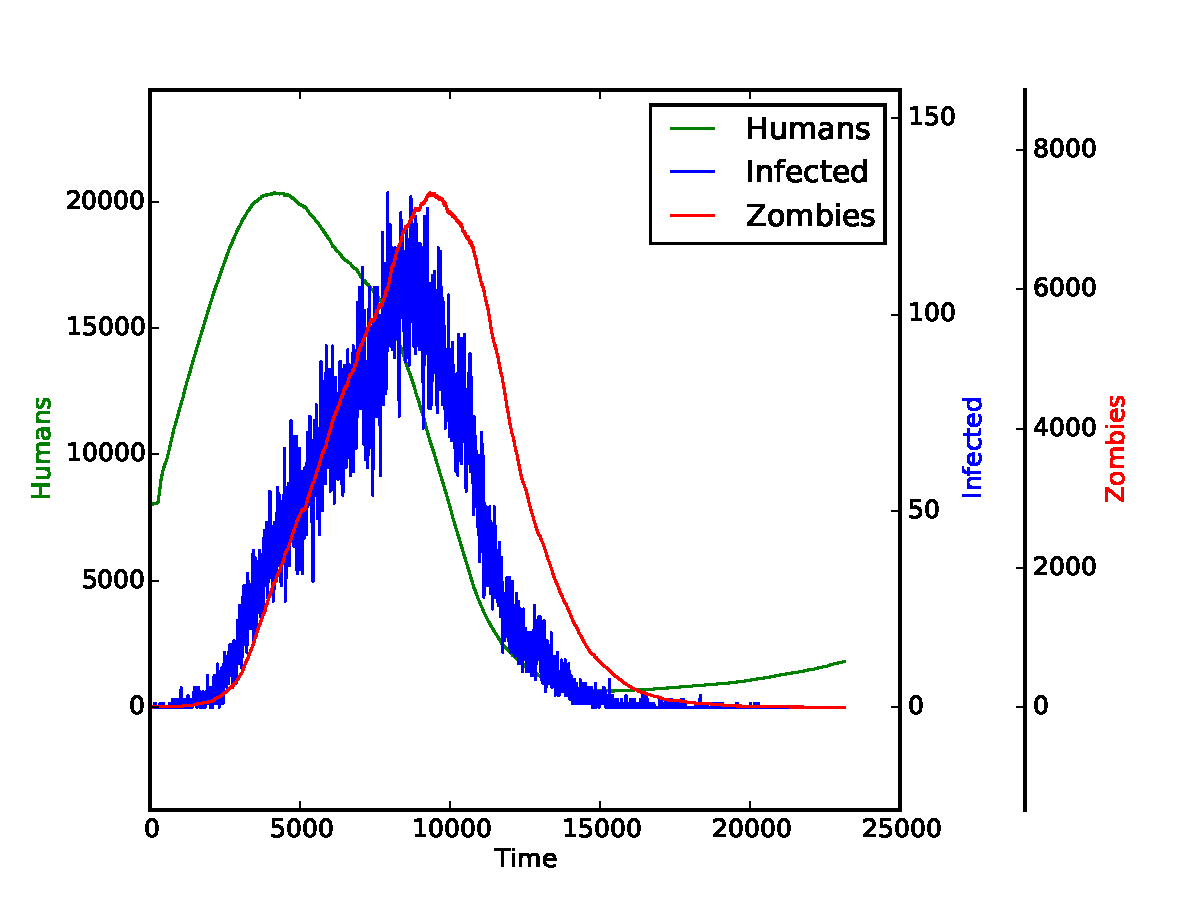
\includegraphics[width=\textwidth]{uncontrolled_birth_8000}
    \caption{Uncontrolled birth with 8000 people and 2 zombies}
\end{figure*}

The natural choice to change was the birth rate, which was first set to be constant.
As there are less humans, the constant birth rate, which works for original population, cannot be used any more.
Humans don't meet as often and therefore their likelihood of making love decrease and their population will as well.
The higher the initial population the more zombies will be created, and the sooner the model will collapse.
We run the simulation starting with only 8000 humans; the failure is clearly visible.
After about only 63 years, zombies died out and human population dropped to 1809 people.
TODO create a new figure

\begin{figure*}[pht]
    \centering
    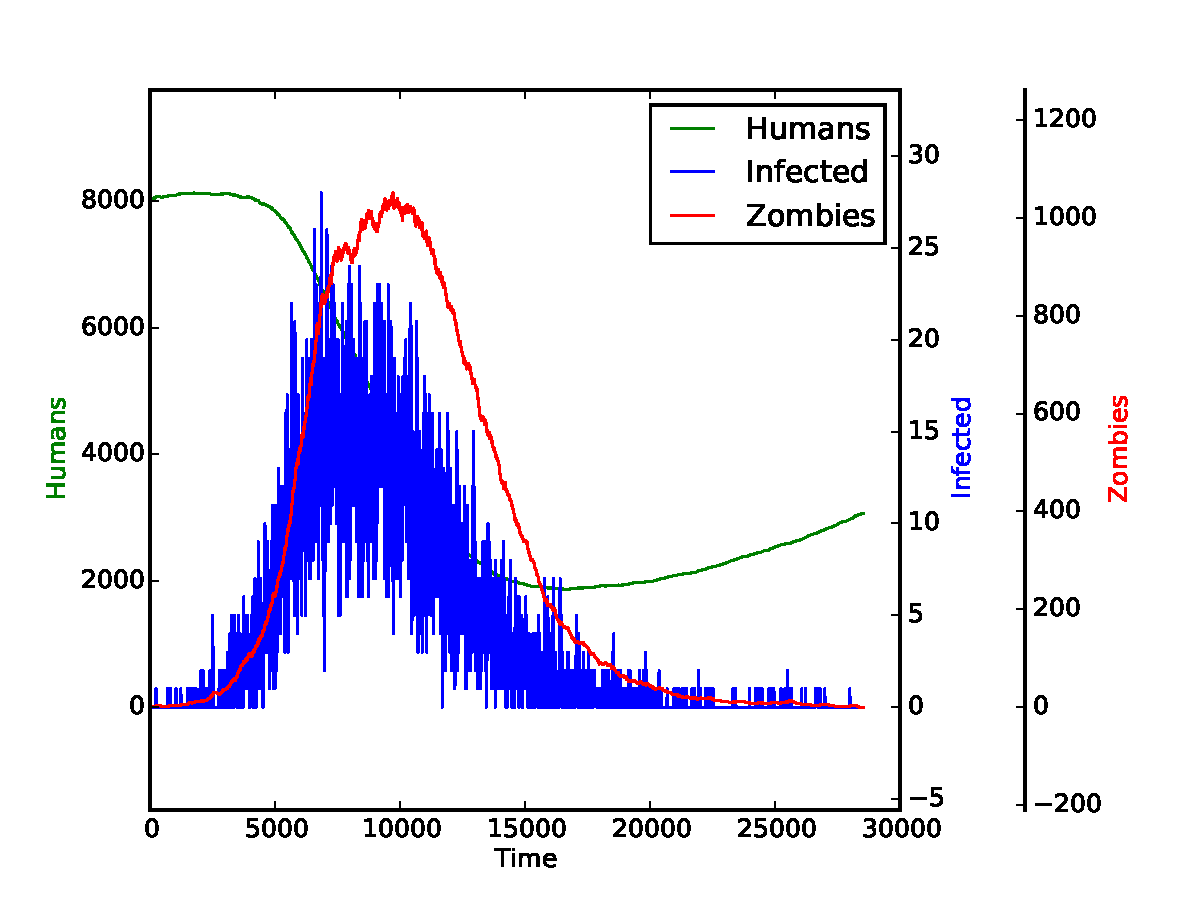
\includegraphics[width=\textwidth]{equal_birth_8000}
    \caption{Equal birth with 8000 people and 2 zombies}
\end{figure*}

The next attempt used the initial birth rate multiplied by a quotient which was defined as a ratio of initial and current population.
As the population drops down, the humans shall reproduce more often and therefore raise back to the original population size.
The model without zombies using this technique is much more stable, however the quotient is not strong enough to deal with zombies.
A simulation starting with 8000 humans is shown in the figure.
Starting with more humans would cause more zombies, and therefore steeper decrease of humans and the eventual lack of human supply would be the reason why zombies would die out quicker.
TODO create a new figure

\subsubsection{Function of densities ratio}

\begin{figure*}[pht]
    \centering
    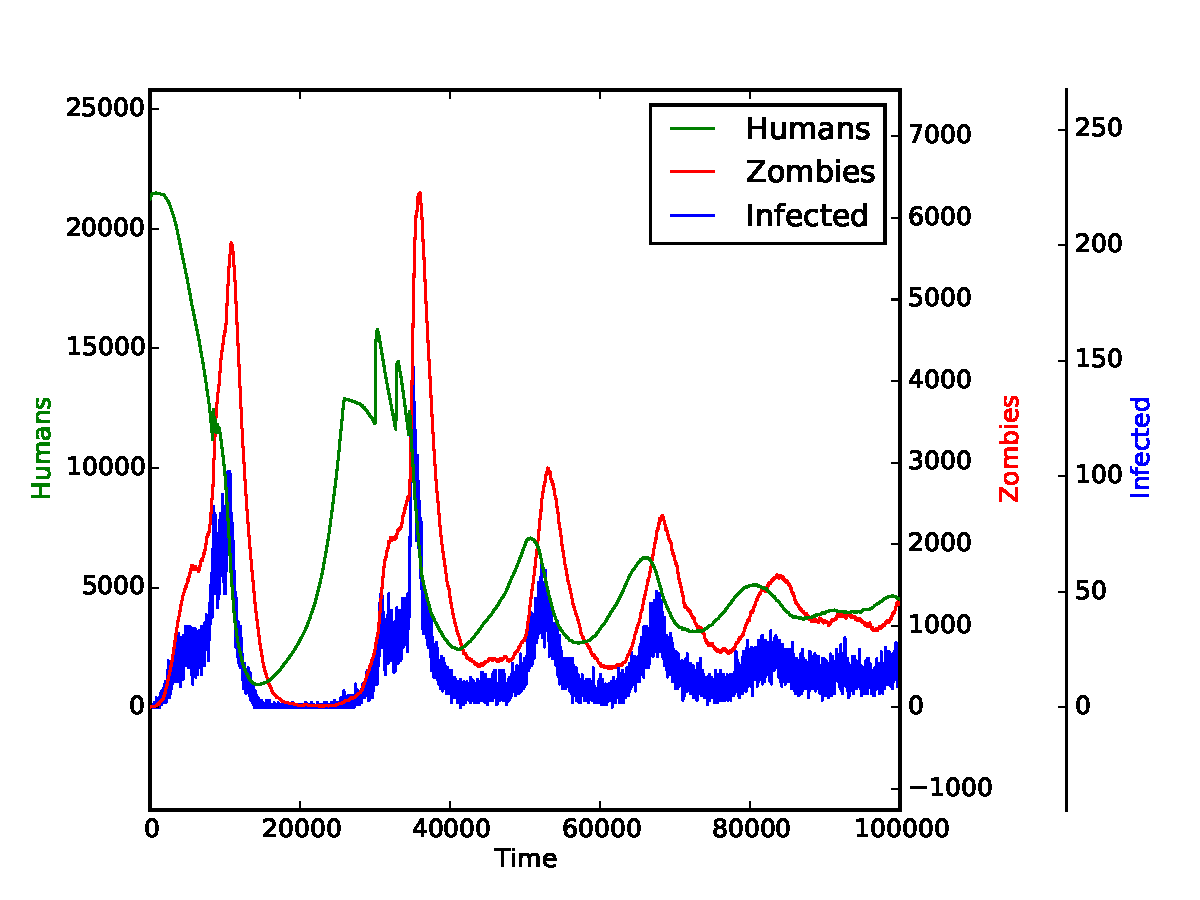
\includegraphics[width=\textwidth]{stable}
    \caption{Stable populations of humans and zombies}
\end{figure*}

The aim of the birth rate function, which depends on population density, is to allow free initial decrease of humans, and then ``kick-in'' when the population is lower.
The initial stage is important because otherwise the population of zombies would become too high and the model would not be stable.
We tried to use several function which has the mentioned properties and also become identity close to initial density.
Our candidate for the quotient function was $r^{const}$, where $r$ is the ratio of population densities.

The optimal value for the constant in exponent, let's call it situation awareness, is 2.5.
Higher values make the populations oscillate in time, and lower values makes the population unnaturally stable.
The population sizes for the full initial human population of 21,250 is shown in the figure.

\begin{figure*}[pht]
    \centering
    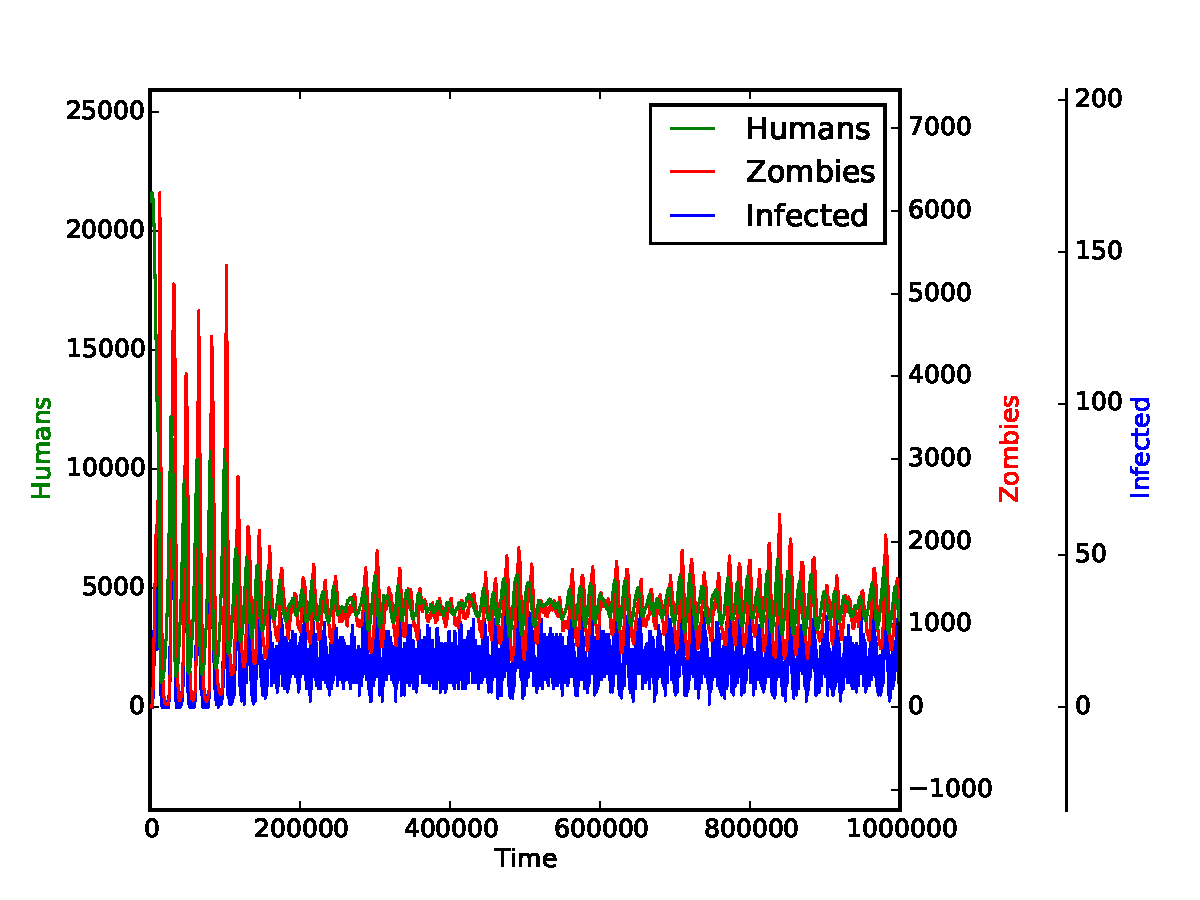
\includegraphics[width=\textwidth]{stable_1000000}
    \caption{2740 years long stable simulation}
\end{figure*}

We have also run the simulation for a longer period to discover its other properties.
As another figure of ten times longer simulation shows, the sizes of populations of human, infected and zombie make 40 years long cycles.
When the simulation starts, the swings of population sizes are smaller and they eventually become constant, non-zero.
It is also interesting that the initial cycle break each into two individual ones.
To this quite stable stage the model gets after 465 years.
TODO correct simulation figure
TODO adjust number according to the figure

\subsection{Demographics}

When the simulation starts, the number of demographics is exactly as described earlier.
There are noticeable four horizontal areas which correspond to age classes.

After 10 years, there demographic situation remains the same, only shifted to the right.
Zombies start to appear and their age distribution starts to spread.

Afert 50 years, after the first zombie peak, which is noticeable by the low number of young zombies and few infected, the demographic distribution has changed.
According to model, more femals are born, however being slower (and having lower daily death probability), their number becomes less than number of males.

After 150 years, the populations have stabilized, there are many infected and the population distributions got their final shape.
This figure is also an example of pregnant infected female.

The situation at the end of the simulation after 100,000 days (appoximately 274 years) is no different from the previous situation.

\begin{figure*}[pht]
    \centering
    \includegraphics[width=0.8\textwidth]{step-000000.png}
    \caption{Simulation mesh at the beginning}
\end{figure*}

\begin{figure*}[pht]
    \centering
    \includegraphics[width=\textwidth]{step-000000.pdf}
    \caption{Demographics at the beginning}
\end{figure*}

\begin{figure*}[pht]
    \centering
    \includegraphics[width=0.8\textwidth]{step-003650.png}
    \caption{Simulation mesh after 10 years}
\end{figure*}

\begin{figure*}[pht]
    \centering
    \includegraphics[width=\textwidth]{step-003650.pdf}
    \caption{Demographics after 10 years}
\end{figure*}

\begin{figure*}[pht]
    \centering
    \includegraphics[width=0.8\textwidth]{step-018250.png}
    \caption{Simulation mesh after 50 years}
\end{figure*}

\begin{figure*}[pht]
    \centering
    \includegraphics[width=\textwidth]{step-018250.pdf}
    \caption{Demographics after 50 years}
\end{figure*}

\begin{figure*}[pht]
    \centering
    \includegraphics[width=0.8\textwidth]{step-053100.png}
    \caption{Simulation mesh after 150 years}
\end{figure*}

\begin{figure*}[pht]
    \centering
    \includegraphics[width=\textwidth]{step-053100.pdf}
    \caption{Demographics after 150 years}
\end{figure*}

\begin{figure*}[pht]
    \centering
    \includegraphics[width=0.8\textwidth]{step-100000.png}
    \caption{Simulation mesh after 274 years}
\end{figure*}

\begin{figure*}[pht]
    \centering
    \includegraphics[width=\textwidth]{step-100000.pdf}
    \caption{Demographics after 274 years}
\end{figure*}

\subsection{Scaling}

\begin{figure*}[ht]
    \centering
    \begin{tabu} {| X[0.8,c,p] || X[1,c,p] | X[1,c,p] | X[1,c,p] |}
        \rowfont{\bfseries}
        \hline
        Threads &
        First attempt &
        Second attempt&
        Third attempt \\
        \hline
        \hline
        \textbf{1} & 180588.734000 & 180633.477000 & 180441.396000 \\
        \hline
        \textbf{2} & 94541.958000 & 95547.356000 & 94704.053000 \\
        \hline
        \textbf{4} & 49689.704000 & 50052.682000 & 50359.165000 \\
        \hline
        \textbf{8} & 25863.988000 & 26373.077000 & 26276.703000 \\
        \hline
        \textbf{16} & 14365.825000 & 14386.286000 & 14363.556000 \\
        \hline
        \textbf{32} & 10598.242000 & 10936.435000 & 10854.121000 \\
        \hline
        \textbf{64} & 14785.381000 & 14363.065000 & 14936.496000 \\
        \hline
    \end{tabu}
    \caption{Scaling depending on number of threads}
\end{figure*}

The model implemented in C using OpenMP, running in several threads.
On Avoca, the IBM Blue Gene/Q supercomputer, a single node provides 16 cores with 4 threads each.
Our model could utilise all 64 threads as most of the simulation does not need any thread synchronisation.

We run the model three times for 1000 iterations in order to ensure the influence of randomness does not make the results odd.
The results are in the table above, running times are in milliseconds.
We expected a perfect scaling up to 16 threads -- each of them will be assigned to a dedicated core.
Running with 32 cores still provides an improvement, but not a significant one.
The drop of performace when running with 64 threads is probably caused by the hardware architecture of the CPU.
In our opinion it is not caused by locking parts of the world as there are still at least 7 columns for each thread (we lock only three of them).

\section{Recommendations}

TODO write recommendation


\begingroup
\raggedright

\bibliographystyle{IEEEtran}
\bibliography{references}
\endgroup

\end{document}

% vim: ft=tex ts=4 sw=4 et
